%%%\documentclass[%
%%%%reprint,
%%%%superscriptaddress,
%%%%groupedaddress,
%%%%unsortedaddress,
%%%%runinaddress,
%%%%frontmatterverbose, 
%%%preprint,
%%%%showpacs,preprintnumbers,
%%%%nofootinbib,
%%%%nobibnotes,
%%%%bibnotes,
%%% amsmath,amssymb,
%%%%aps,
%%%%pra,
%%% prb,
%%%%rmp,
%%%%prstab,
%%%%prstper,
%%%floatfix,
%%%%nolongbibliography
%%%]{revtex4-1}

\documentclass[review,12pt]{elsarticle_summary_report}
\usepackage[top=1.0in, bottom=1.0in, left=1in, right=1in]{geometry}


%%%%%%%%%%%%%%%%%%%%
%\usepackage{amsfonts}
%\usepackage{amssymb}
%\usepackage{MnSymbol}
\usepackage{graphicx}
\usepackage{courier}
\usepackage{psfrag}
\usepackage{amsmath}
\usepackage[usenames]{color}
\usepackage{leftidx}
\usepackage[small]{subfigure}
\usepackage{stmaryrd}
\usepackage{amsthm}
\usepackage{multirow}
\usepackage[table]{xcolor}
% \usepackage{natbib}
\usepackage{nomencl}
\usepackage{setspace}
\usepackage{dcolumn}% Align table columns on decimal point
\usepackage{bm}% bold math
\usepackage{pdflscape}
% \usepackage{showkeys}
%%%%%%%%%%%%%%%%%%%%

\usepackage{hyperref}
\hypersetup{
    colorlinks=true,
    linkcolor=blue,
    filecolor=magenta,      
    urlcolor=cyan,
}

% \usepackage[active,tightpage]{preview}
% \PreviewSnarfEnvironment[{[]}]{figure}

\makenomenclature

\graphicspath{ {./Figures/cav_17_results/}
               {./Figures/pillbox_coarse_uniform_results/}   
               {./Figures/geom_inquires_impl/}   
             }

%\renewenvironment{equation}[0]{equation}{equation}

%%%%%%%%%%%%%%%%%%%% Additional Commands
%%%%%%%%%%%%%%%%%%%%
%\numberwithin{equation}{section}  	%%Equation Numbering
%%%%%%%%%%%%%%%%%%%%
\begin{document}

\title{PROGRESS REPORT}% Force line breaks with \\
%\thanks{}%

\author[]{Morteza H. Siboni \\
Gerrett Diamond \\
Cameron W. Smith}
%\ead{email address}

%\author[inst1]{Corresponding Author \corref{cor1}}
%\cortext[cor1]{Corresponding author}
%\ead{ca@email.host.edu}
%\address[inst1]{Department of Mechanical Engineering and Applied Mechanics, University of Pennsylvania, \\ Philadelphia, PA 19104-6315, USA}


\date{\today}



% \begin{abstract}
%   In this document we provide an update on the current status of the Omega3P project. In particular, the following topics will be addresses: (a) In-memory mesh integration and load balancing, (b) the parallel adaptive loop, and (c) the implementation details for replacing the geometry calls in Omega3P  with the corresponding PUMI calls.
% \end{abstract}

% \begin{keyword}
% \end{keyword}

\maketitle


% \begin{spacing}{0.5}
% \printnomenclature
% \end{spacing}


\section{Introduction}
In this report, we provide some details on the state of the Omega3P project. In particular, Sec. \ref{load_balance} describes what has been done for partitioning and load balancing. Section \ref{in_memory} provides the details of in-memory mesh integration. In Sec. \ref{adaptive_loop} we discuss the details of the adaptive loop implementation and provide some example results. Finally, Sec. \ref{high_order_geom} provides a quick overview of the steps taken towards moving to higher-order geometric meshes.

\section{\label{load_balance}Load Balancing}
In each iteration of the mesh adaptation loop a new partition is generated on the
pumi-mesh before converted over to the slac-mesh. The initial partition is generated
using Zoltan's graph partitioning. Then SCOREC's ParMA, partitioning using mesh adjacencies,
is used to perform load balancing by iterative diffusion. ParMA's multi-entity balancing
traverses an application-specified priority list of entity orders (vertex, edge, face,
region) to balance in descending order.
For each entity order iterative diffusion is executed until balance is reached
or no further improvement is possible.

ParMA's support for multi-entity balancing was extended for Omega3P's needs.
The Omega3P solving step relies on both on-part mesh entities as well as a layer
of ghosted elements along each part boundary.
Omega3P's ghosting uses vertex adjacency such that every element that shares a
vertex with a part boundary will be ghosted to each part that shares that
boundary.
This can be seen in Figure \ref{fig:ghost3} that shows an example of a mesh with
a layer of ghosting.
In order to improve Omega3P's performance and scalability, ParMA targets
minimizing the sum of the ghosted and on-part elements as well as the mesh
entities holding degrees-of-freedom.

\begin{figure}[ht]
\centering
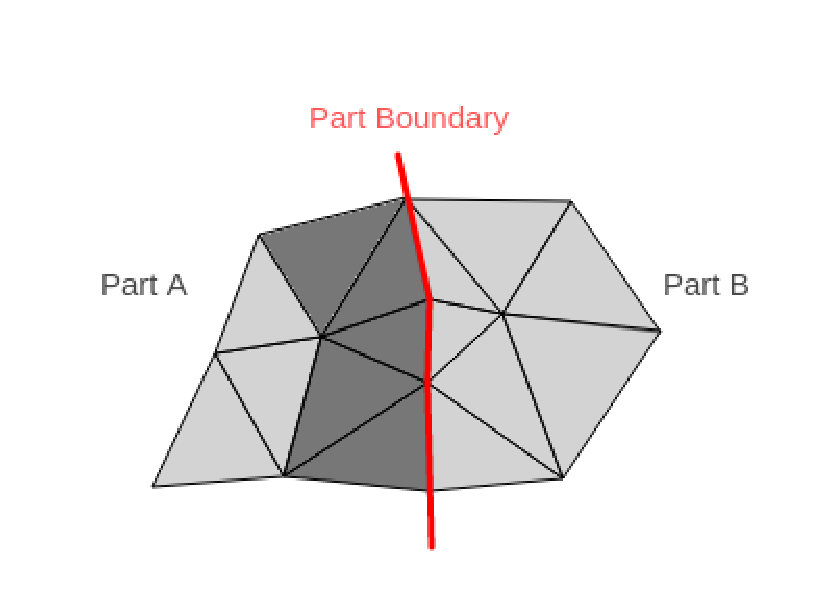
\includegraphics[width=0.6\textwidth]{ghost.eps} 
\caption{\label{fig:ghost3} A layer of ghosted elements from part A to part B. The darker elements represent all the elements on part A that part B will copy to create its remote mesh.}
\end{figure}

ParMA balances the degree-of-freedom holders defined by 
hierarchical Nedelec basis functions~\cite{ko2010advances,ingelstrom2006new} by
reusing existing multi-entity target and boundary-element selection
procedures.
For first order elements this requires balancing edges.
Second order elements requires edges and faces, and above that edges, faces, and
regions need to be balanced.
Each of these entity balancing procedures accounts for the ghosted weight
contribution by performing an additional neighborhood
exchange~\cite{ibanez2014hybrid} of the exact weight of ghosted layer entities.
Thus ParMA can readily account for balancing the work load, in terms of number
of equations per-part, for p-version finite elements by setting mesh entity
weights based on the different entity p-orders.


%need to add results on the load balancing from old report

\section{\label{in_memory}Fully Parallel In-Memory Mesh Integration}
In order to achieve high performing and scalable component interactions between
Omega3P and PUMI we avoid
file-based I/O through in-memory data streams and component functional
interfaces. Towards complete support of the solve-adapt cycle we have implemented in-memory
procedures to convert Omega3P meshes and fields to and from  PUMI data structures.
The key advantage of this approach is the small amount of relatively simple code
required; we simply needed to read and write the Omega3P mesh and field
structures.
A similar PUMI in-memory integration with the Albany Multiphysics
framework~\cite{salinger2013albany,Albany2015} reduced the data transfer time
required to support an adaptive step on a 22 million element mesh from over 100
seconds using files to 23 seconds on 1024 cores.

Mesh conversion begins with a version of Omega3P's NetCDF file reader that is altered
to read the mesh data into PUMI data structures instead of Omega3P's Distmesh. With 
the PUMI mesh we are able to perform partitioning and load balancing as well as adaptation 
while only storing the PUMI mesh. After we have a finalized PUMI mesh a second 
overloaded version of Omega3P's file reader is used to convert the PUMI mesh to 
Omega3P's DistMesh. This is done by using the data from the in-memory PUMI mesh as the 
input instead of the NetCDF file. After the conversion to DistMesh, we store both the
PUMI Mesh and the Omega3P DistMesh for the duration of the finite element setup and 
computations. The time required to convert from the PUMI parallel mesh to the
parallel DistMesh requires less than 0.1\% of the total execution time.
Adaptive simulations will call the PUMI-to-DistMesh conversion routine every
solve-adapt cycle after executing PUMI mesh adaptation and load balancing.
We have demonstrated a low runtime and memory overhead implementation for the
PUMI-to-DistMesh conversion which ensures that it is not a bottleneck
in these simulations.

%Memory images to be added

\clearpage
\newpage

\section{\label{adaptive_loop}The Adaptive Loop}
At this stage, we have the adaptation loop in place which consists of the following steps:

\setstretch{0.75}
\begin{itemize}
  \item[] \texttt{while not converged \{ }
   \begin{itemize}
     \item \texttt{partition the mesh using ParMA with a focus of owned and ghost elements}
     \item \texttt{convert PUMI-mesh to SLAC-mesh}
     \item \texttt{run the appropriate Omega3P eigensolver}
     \item \texttt{transfer electric field values to the PUMI-mesh}
     \item \texttt{check for convergence}
     \item \texttt{run Super-convergent Patch Recovery (SPR) -> error estimation -> size field}
     % \item \texttt{convert 2nd order Lagrange to 2nd order Bezier}
     \item \texttt{run the curve adapt}
     % \item \texttt{convert 2nd order Bezier back to 2nd order Lagrange}
   \end{itemize}

 \item[] \texttt{  \} }
\end{itemize}
\setstretch{1.5}
It is important to emphasize that, the current adaptive loop improves upon the previously available adaptive loop (implemented by Kai) in that it is fully parallel. Recall that the previous implementation required repartitioning a serial mesh after parallel adaptation.


\subsection{Results for the Adaptive Loop}
Figures \ref{pill} and \ref{cav} show two working examples for the current curve adaptation loop.
\begin{landscape}
\begin{figure}[ph!]
\centering
\subfigure[]{\label{pill_init}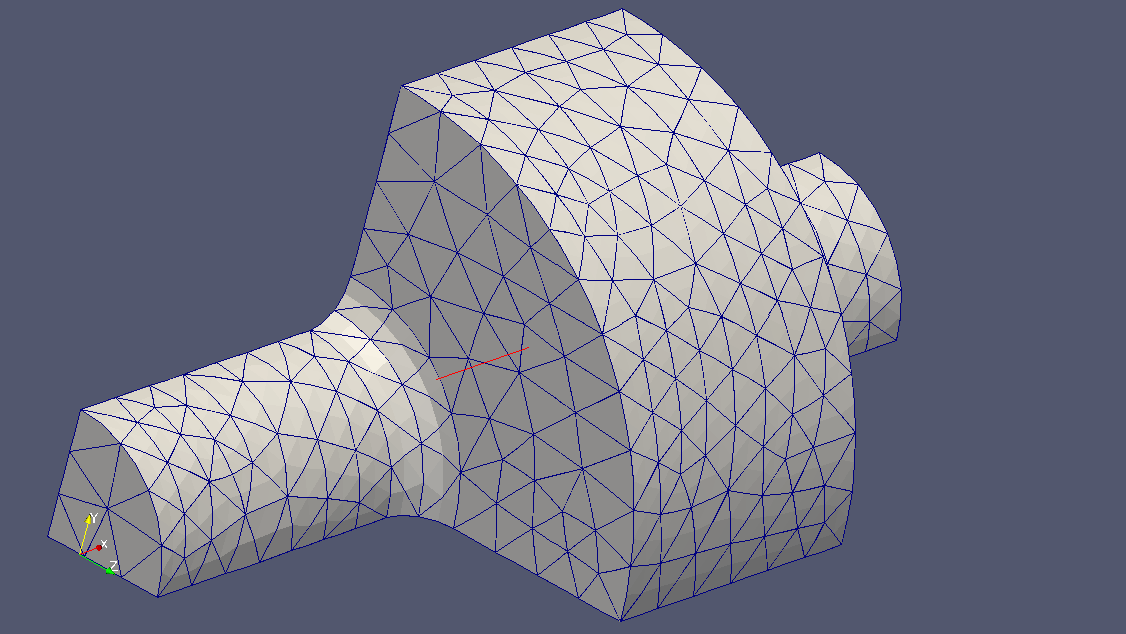
\includegraphics[width=0.55\textwidth]{al_0_ar_0p0125_3721_elems.png}}
\hspace*{50pt}
\subfigure[]{\label{pill_size}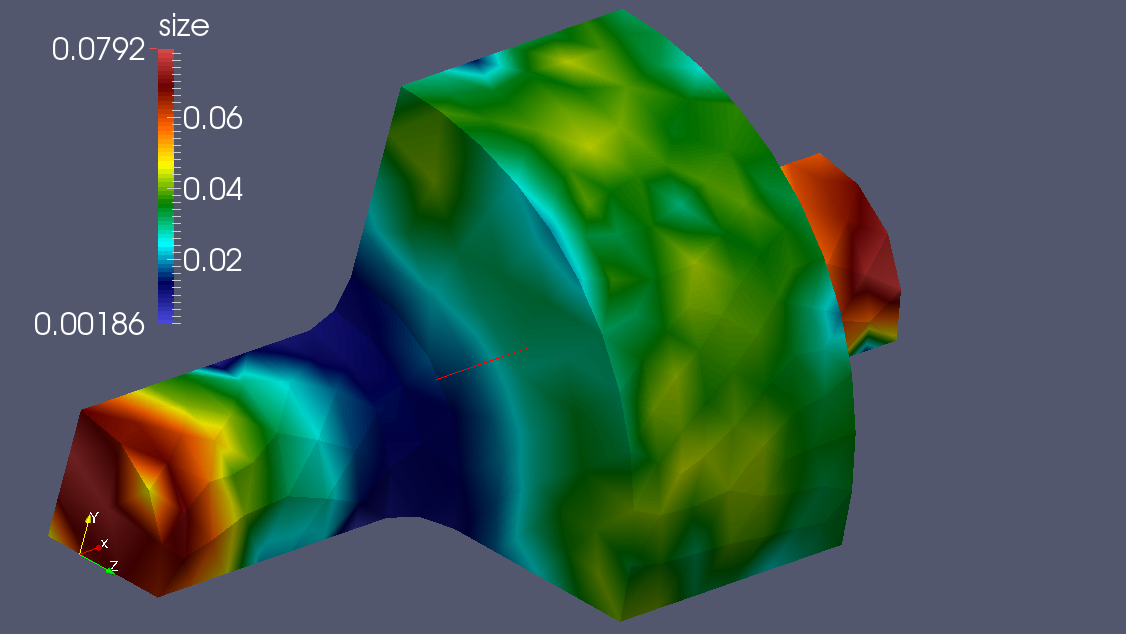
\includegraphics[width=0.55\textwidth]{al_0_ar_0p0125_3721_elems_size_field.png}}
\\
\subfigure[]{\label{pill_adapt}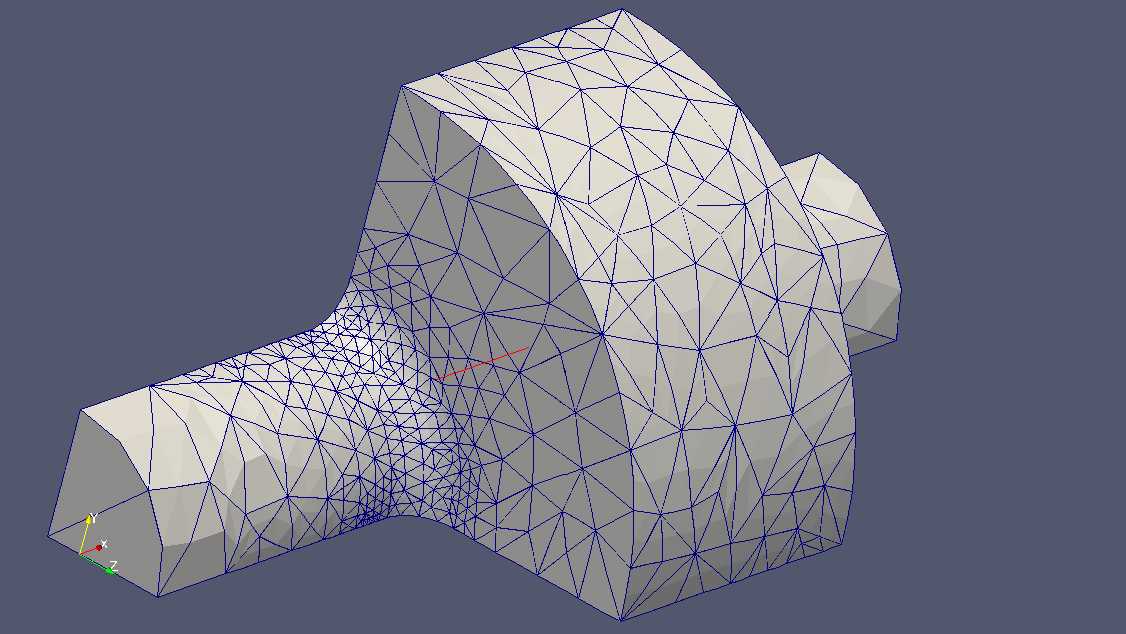
\includegraphics[width=0.55\textwidth]{al_3_ar_0p0125_14221_elems.png}}
\hspace*{50pt}
\subfigure[]{\label{pill_field}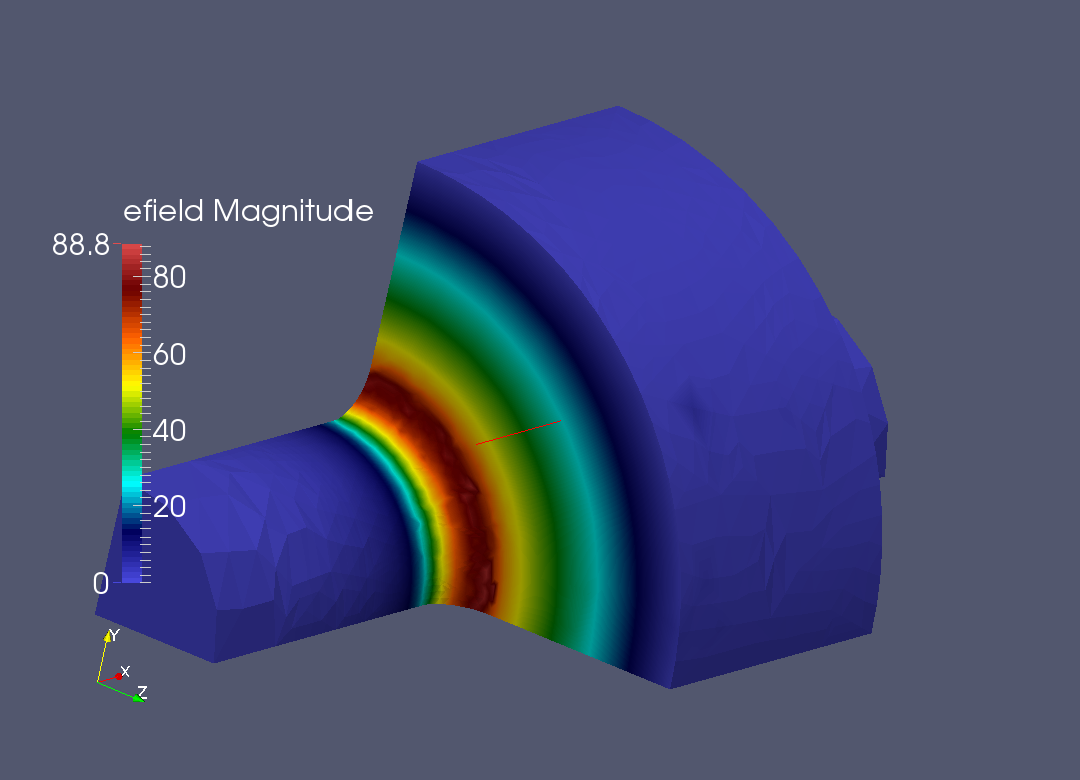
\includegraphics[width=0.55\textwidth]{al_3_ar_0p0125_14221_elems_e_field.png}}
\caption{\label{pill} This Figure shows the results for the PILLBOX model. (a) shows the initial mesh [$\sim3.7\text{K}$ elements], (b) shows the initial size-field, (c) shows the adapted mesh after 3 adaptation steps [$\sim14\text{K}$ elements], and (d) shows the electric field for the final adapted mesh.}
\end{figure}
\end{landscape}
\begin{landscape}
\begin{figure}[ph!]
\centering
\subfigure[]{\label{cav_init}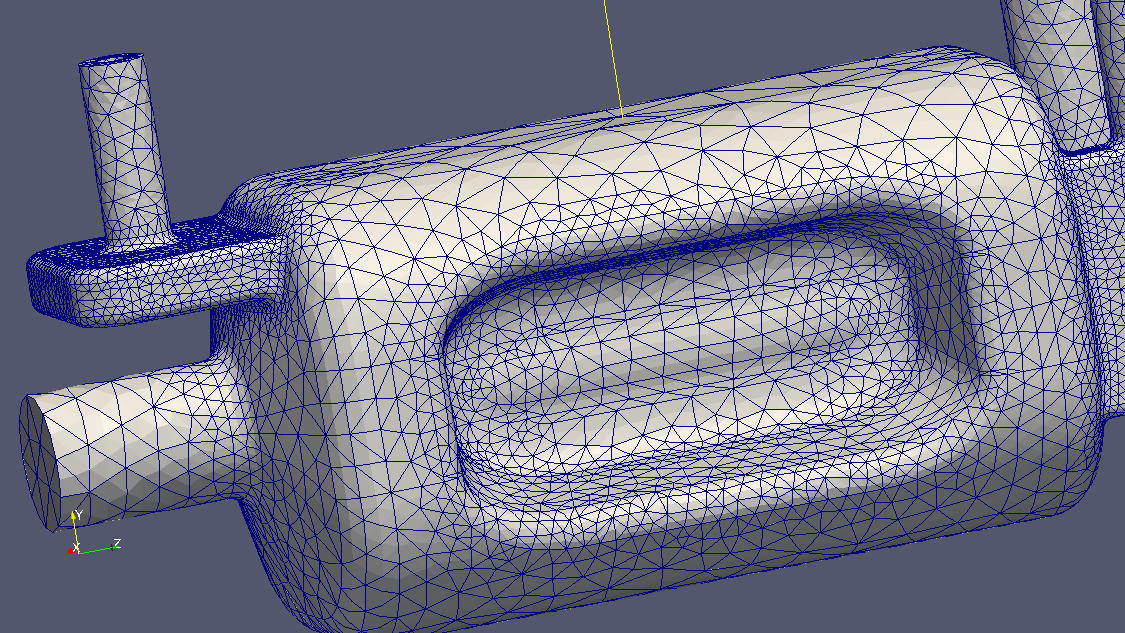
\includegraphics[width=0.55\textwidth]{al_0_ar_0p0125_126044_elems.png}}
\hspace*{50pt}
\subfigure[]{\label{cav_size}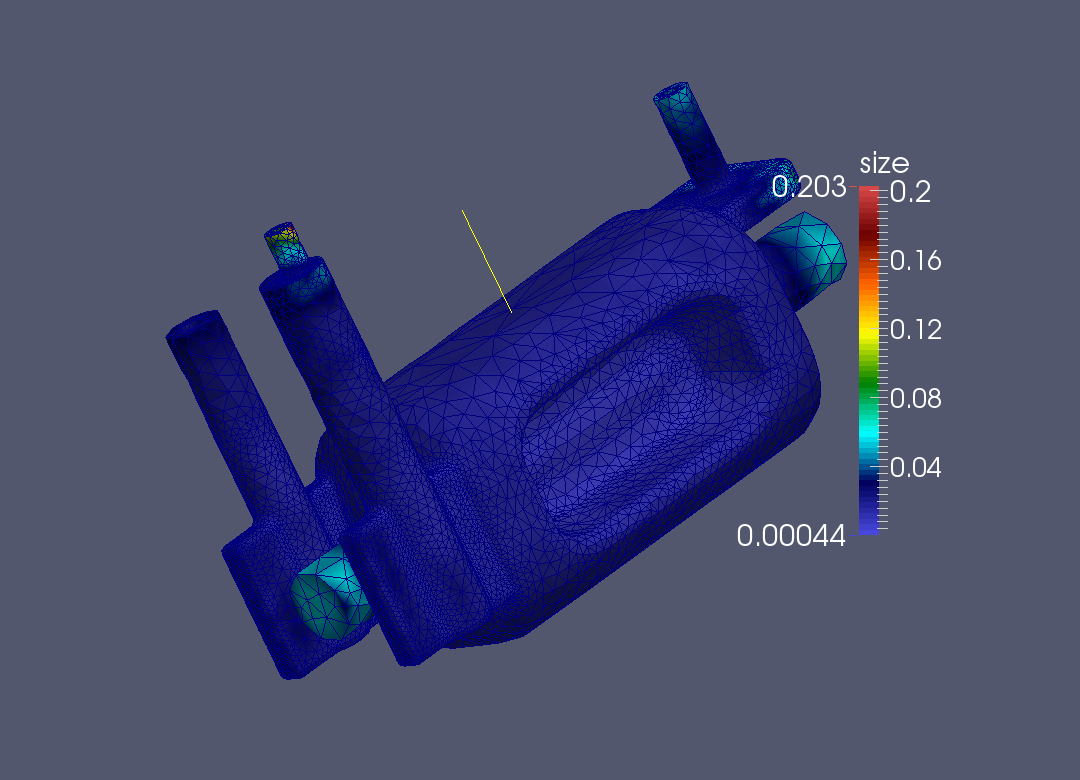
\includegraphics[width=0.55\textwidth]{al_0_ar_0p0125_126044_elems_size_field.png}}
\\
\subfigure[]{\label{cav_adapt}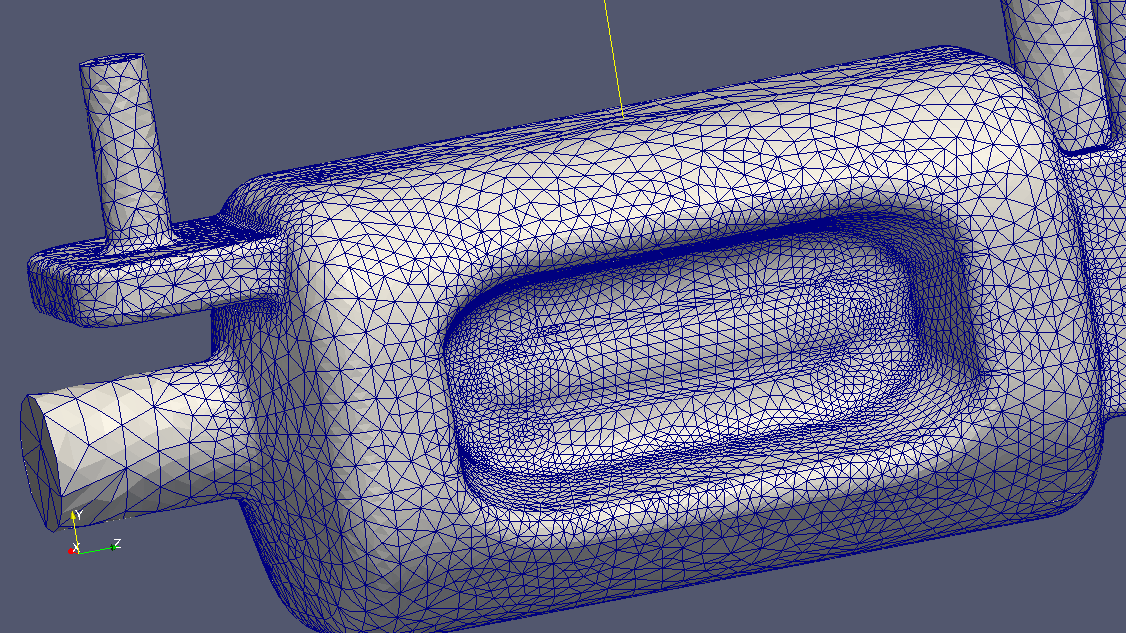
\includegraphics[width=0.55\textwidth]{al_3_ar_0p0125_386896_elems.png}}
\hspace*{50pt}
\subfigure[]{\label{cav_field}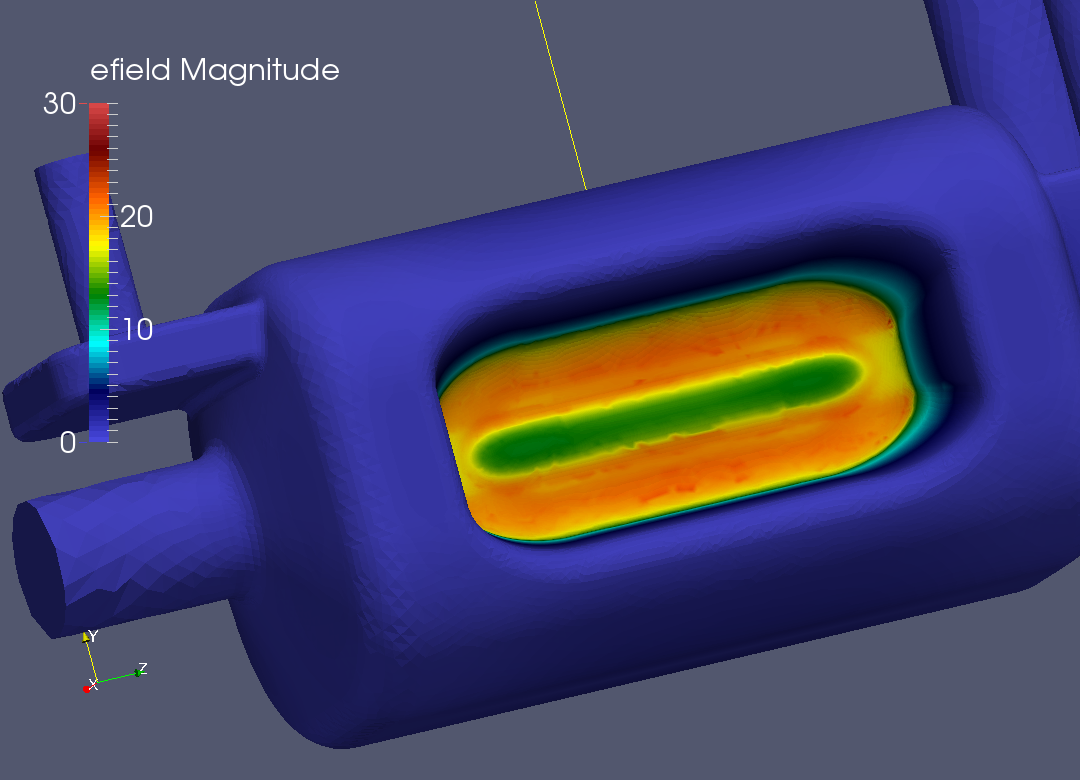
\includegraphics[width=0.55\textwidth]{al_3_ar_0p0125_386896_elems_e_field.png}}
\caption{\label{cav} This Figure shows the results for the CAV17 model. (a) shows the initial mesh [$\sim126\text{K}$ elements], (b) shows the initial size-field, (c) shows the adapted mesh after 3 adaptation steps [$\sim380\text{K}$ elements], and (d) shows the electric field for the final adapted mesh.}
\end{figure}
\end{landscape}
In particular, Fig. \ref{pill} shows the results for the smaller ``PILLBOX''. We start with a uniform and relatively coarse mesh as shown in Fig. \ref{pill_init}. The desired size field for this initial mesh is obtained based on the magnitude of the electric filed and it is shown in Fig. \ref{pill_size}. The final, adapted mesh (for this specific example we needed 3 levels of adaptation) is shown in Fig. \ref{pill_adapt}. Figure \ref{cav} shows the corresponding result for the larger ``CAV17'' model.


\section{\label{high_order_geom}Moving Towards Higher-Order Geometries}

In order to be able to increase the order of the finite element basis functions to exploit the exponential convergence rate of the p-version finite elements, one needs to also increase the geometric order of the elements near the curved boundaries. Otherwise, the error in the geometric representation of such curved elements prevents the exponential growth rate in the p-version finite element \cite{LuoShephard_04, DeyShephard_97, LuoShephard_02}.

As a first step towards using higher-order geometric elements, we have been able to replace the Omega3P calls to compute determinant of the Jacobian with the corresponding PUMI calls. This is done by storing and additional pointer in each Omega3P-element that points to the corresponding  PUMI-element (see Fig. \ref{imp} for the details of the implementation).
\begin{figure}[ph!]
\centering
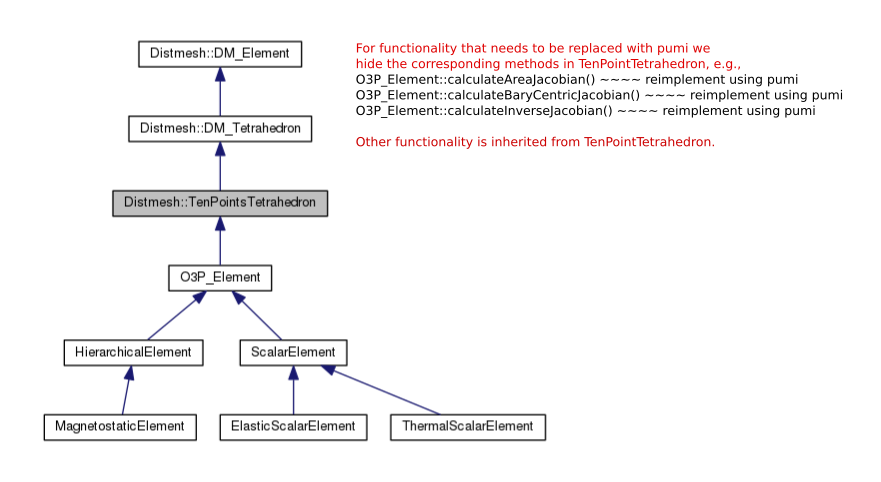
\includegraphics[width=0.95\textwidth]{hide_ten_point_tet.png}
\caption{\label{imp} This Figure shows the implementation details for replacing Omega3P calls for determinant calculation with the corresponding PUMI calls.}
\end{figure}
This, in theory, should make it possible to raise the (geometric) order of the elements to higher that quadratic. (Currently, we have support for up to 6th order Bezier elements in PUMI.)


\section*{References}
% \bibliographystyle{elsarticle-harv_noURL}
\bibliographystyle{plain}
\bibliography{scorec-refs/partition,scorec-refs/meshdb,scorec-refs/hardware,scorec-refs/io,scorec-refs/frameworks,scorec-refs/cr,scorec-refs/fem,scorec-refs/meshgen,scorec-refs/msgpass,geometry}


\end{document}
